

\newpage
\begin{center}
	\textbf{\large ГЛАВА 1 \\ ПОСТАНОВКА ЗАДАЧИ И ПЛАН РЕШЕНИЯ}
\end{center}
\refstepcounter{chapter}


% \section*{}
\addcontentsline{toc}{chapter}{ГЛАВА 1}
\section{Анализ существующих моделей шагающих роботов}

Автономных роботов можно условно разделить на две категории: стационарные роботы и мобильные роботы. Одним из типов стационарных робототехнических систем является манипулятор, который размещает поверхностно установленные компоненты с чрезвычайно высокой точностью\cite{bibl1}, т.е. в сборочной линии, рука робота способна перемещаться с высокой скоростью и точностью для выполнения повторяющихся задач, таких как точечная сварка\cite{welding} и покраска\cite{painting}. Другим важным типом стационарных роботизированных систем является устройство схвата\cite{grab}, которое обычно используется для захвата нужных объектов. В настоящее время разработано множество роботизированных механических устройств имитирующие руки и пальцы, которые широко применяются,например, в сельском хозяйстве\cite{farming}. К сожалению, эти стационарные роботы страдают от недостаточной подвижности и ограниченного диапазона движения. В отличие от них, мобильные роботы способны передвигаться по пересеченной местности. Благодаря гибкости мобильных роботов, они широко применяются во многих областях, таких как строительство, охрана объектов, сбор информации. В этих сценариях применения мобильные роботы могут быть классифицированы на наземные, воздушные и подводные. Кроме того, в соответствии с различными механическими структурами, наземных роботов можно разделить на колесные, гусеничные и шагающие роботы, соответственно.

В ситуациях неровной местности для реализации локомоции больше подходят шагающие роботы, в силу их способности адаптироваться к местности. Кроме того, они также могут применяться областях, далеких от промышленности, например медицина \cite{medicine1,medicine2} и образование \cite{edu}. Таким образом, шагающие роботы стали актуальной темой для исследований в области робототехники, благодаря их преимуществу перед колесными и гусеничными роботами.

Рассмотрим несколько моделей шагающих роботов, на основе которых проведем анализ конструкции (раздел \ref{C1_2}).

Mini Cheetah \cite{cheetah} - это четырехногий робот, разработанный в Массачусетском технологическом институте (рисунок \ref{cheetah}). Основное внимание в роботе уделяется его модульным приводам высокой мощности. Mini Cheetah обладает двенадцатью одинаковыми приводами, которые состоят из бесщеточного двигателя, планетарного редуктора с передаточным числом 6:1, энкодера и контроллера двигателя. Все приводы Mini Cheetah обмениваются данными по единой шине CAN-bus.
\begin{figure}[h!]
	\begin{center}
		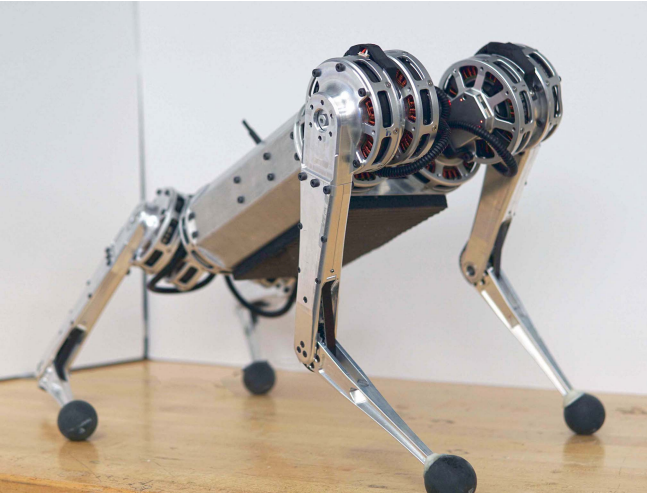
\includegraphics[width=0.5\textwidth]{cheetah}
		\caption{Mini Cheetah, разработанный в MIT}
		\label{cheetah}
	\end{center}
\end{figure}

Stanford Doggo\cite{SDoggo} - квази-прямоходящий четырехногий робот, разработанный в Стэнфорде. Он обладает очень высокой выходной мощностью по сравнению с его весом и низкой ценой. Такой высокий крутящий момент достигается за счет квазипрямого привода и меньшего количества степеней свободы на каждой ноге.
\newpage
\begin{figure}[h!]
	\begin{center}
		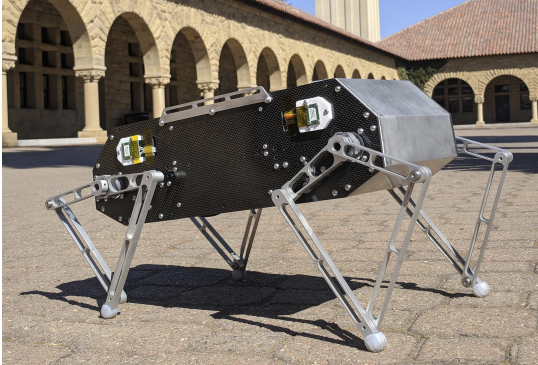
\includegraphics[width=0.5\textwidth]{SDoggo}
		\caption{Stanford Doggo, разработанный в Стэнфордском университете}
		\label{SDoggo}
	\end{center}
\end{figure}

Spot\cite{spot} - шагающий робот, разработанный компанией Boston Dynamics, представляет из себя четвероногого робота, предназначенного для промышленного рынка. По этой причине он обладает более широкими возможностями, чем другие четвероногие роботы, так как создан для выполнения бизнес задач. Он обладает хорошей подъемной силой, имеет возможность установки дополнительных датчиков и инструментов на верхней части корпуса, а также использует камеру для технического зрения с целью сканирования окружающей обстановки.
\begin{figure}[h!]
	\begin{center}
		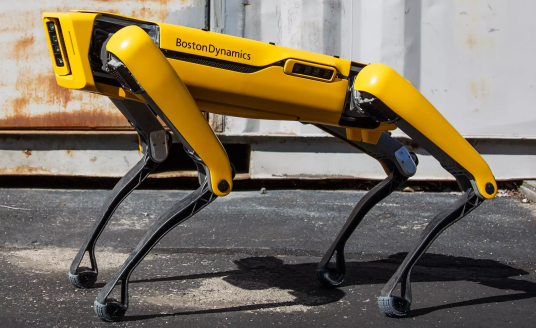
\includegraphics[width=0.5\textwidth]{spot}
		\caption{Spot, разработанный в компании Boston Dynamics}
		\label{spot}
	\end{center}
\end{figure}


\section{Задачи работы}\label{C1_1}

Создание функционирующего прототипа шагающего робота, приближенного к промышленным моделям, является существенно сложным и дорогостоящим процессом. В связи с этим, для достижения поставленных целей, в данной работе будут применены упрощения, которые окажут влияние на некоторые технические аспекты, однако не повлекут за собой потерю общей ценности исследования - разработки действующего прототипа с готовым управлением, полученным путем решения задач механики и управления без использования методов искусственного интеллекта.


%Задача создания работоспособного прототипа шагающего робота близкого к промышленным образцам является очень сложной и одновременно дорогостоящей работой. По этой причине в рамках работы будут использоваться упрощения, которые повлияют на некоторые технические особенности, но не изменят общей ценности работы – разработки работоспособного прототипа с готовым управлением, полученным путем решения задач механики и управления без применения искусственного интеллекта.
 
Для выполнения данной работы потребуется:
\begin{itemize}
	\item Разработать кинематическую схему ноги робота.
	\item Разработать общую кинематическую схему робота.
	\item Решить обратную задачу кинематики для положения ноги.
	\item Решить задачу описания модели походки робота.
	\item Разработать твердотельную модель ног и корпуса робота.
	\item Подобрать необходимые сервоприводы в сочленения ног робота.
	\item Подобрать комплектующие, связанные с реализацией контроля сервоприводами.
	\item Разработать программное обеспечение для дистанционного управления роботом.
\end{itemize}
\section{Исследование особенностей строения робота}\label{C1_2}
Среди всех компонентов робота, ноги являются наиболее важными составляющими. Такие свойства, как вес, размеры и приведение в действие суставов, непосредственно влияют на производительность движения ног и, следовательно, точность позиционирования робота.

У упомянутых ранее моделей роботов схожи комплекции как корпуса, так и ног, даже общие объемы роботов будут схожи. 
Каждая нога состоит из тазобедренного сустава, бедра, коленного сустава, голени и стопы для контакта с землей, то есть все ноги обладают тремя степенями свободы, а принципы расположения двигателей в ногах имеют минимальное расхождение. Это следствие того, что промышленные модели сделаны из металла и действительно требуют расположения тяжелых двигателей как можно ближе к корпусу для большей устойчивости и меньших затрат на управление. 

В рамках данной работы, робот не обладает существенным весом, а также большими размерами корпуса и ног, в следствие чего будут следующие упрощения:
\begin{itemize}
	\item На одну ногу будет две степени свободы, вместо устоявшегося стандарта в виде трех степеней.
	\item Двигатели будут располагаться в области бедра (у корпуса) и колена (в сочленении ног), так как робот обладает небольшой массой и малыми габаритами для классического решения (рисунок \ref{kinematic}).
\end{itemize}


Последующие упрощения могут привести к утрате возможности контролировать отклонения бедра, что в свою очередь подчеркивает необходимость разработки методов компенсации устойчивости при изменениях углов ориентации корпуса в плоскостях крена и тангажа.
\newpage
\begin{figure}[h]
	\begin{center}
		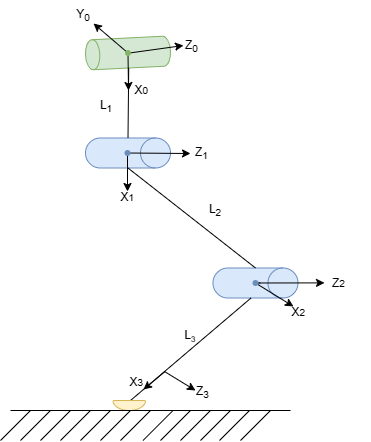
\includegraphics[width=0.6\textwidth]{kinematic}
		\caption{Расположения двигателей для случая трех степени свободы на ногу}
		\label{kinematic}
	\end{center}
\end{figure}
